% !TEX root = C:\Users\panen\MS2\ms2.tex
\documentclass[14pt,a4paper]{scrartcl}
%\documentclass[14pt,a4paper]{article}
\usepackage[T1,T2A]{fontenc}
\usepackage[utf8]{inputenc}
\usepackage{ragged2e}
\usepackage[english,ukrainian]{babel}
\usepackage{misccorr,color,ragged2e,amsfonts,amsthm,graphicx,systeme,amsmath,mdframed,lipsum}
\usepackage{tikz}
\usepackage{esvect}
\usepackage{graphicx}
\usepackage{slashbox}
\usepackage{diagbox}
\usepackage{float}
\usepackage{comment}
\usepackage{amsmath}
\usepackage{alltt}
\usepackage{ amssymb }
\usepackage[unicode]{hyperref}
%\usepackage{biblatex}
%\graphicspath{ {C:\Users\panen\CW_1_Probalility} }
\renewcommand\qedsymbol{$\blacksquare$}
\renewcommand*{\proofname}{\text{Доведення}}
\theoremstyle{definition}
\newtheorem{defo}{Означення}[section]
\newtheorem*{teo}{Теорема}
\newtheorem*{example}{Приклад}
\theoremstyle{remark}
\newtheorem*{remark}{Зауваження}
\theoremstyle{definition}
\newtheorem*{consequence}{Наслідок}
\theoremstyle{definition}
\newtheorem{statement}{Утверждение}[section]
\newmdtheoremenv{boxteo}{Теорема}[section]
%\setlength\parindent{0pt}
\usepackage{lipsum}
\setlength{\parindent}{5ex}
\DeclareMathOperator*\lowlim{\underline{lim}}
\DeclareMathOperator*\uplim{\overline{lim}}
\setcounter{subsection}{-1}
\usepackage{tabularx}


% Default fixed font does not support bold face
\DeclareFixedFont{\ttb}{T1}{txtt}{bx}{n}{12} % for bold
\DeclareFixedFont{\ttm}{T1}{txtt}{m}{n}{12}  % for normal

% Custom colors
\usepackage{color}
\definecolor{deepblue}{rgb}{0,0,0.5}
\definecolor{deepred}{rgb}{0.6,0,0}
\definecolor{deepgreen}{rgb}{0,0.5,0}

\usepackage{listings}

% Python style for highlighting
\newcommand\pythonstyle{\lstset{
language=Python,
basicstyle=\ttm,
otherkeywords={self},             % Add keywords here
keywordstyle=\ttb\color{deepblue},
emph={MyClass,__init__},          % Custom highlighting
emphstyle=\ttb\color{deepred},    % Custom highlighting style
stringstyle=\color{deepgreen},
frame=tb,                         % Any extra options here
showstringspaces=false            %
}}

\definecolor{javared}{rgb}{0.6,0,0} % for strings
\definecolor{javagreen}{rgb}{0.25,0.5,0.35} % comments
\definecolor{javapurple}{rgb}{0.5,0,0.35} % keywords
\definecolor{javadocblue}{rgb}{0.25,0.35,0.75} % javadoc

\lstset{language=C++,
basicstyle=\ttfamily,
keywordstyle=\color{javapurple}\bfseries,
stringstyle=\color{javared},
commentstyle=\color{javagreen},
morecomment=[s][\color{javadocblue}]{/**}{*/},
numbers=left,
numberstyle=\tiny\color{black},
stepnumber=2,
numbersep=10pt,
tabsize=4,
showspaces=false,
showstringspaces=false}


% Python environment
\lstnewenvironment{python}[1][]
{
\pythonstyle
\lstset{#1}
}
{}

% Python for external files
\newcommand\pythonexternal[2][]{{
\pythonstyle
\lstinputlisting[#1]{#2}}}
\usepackage{relsize}
% Python for inline
\newcommand\pythoninline[1]{{\pythonstyle\lstinline!#1!}}
%
% \begin{python}
% class MyClass(Yourclass):
%     def __init__(self, my, yours):
%         bla = '5 1 2 3 4'
%         print bla
% \end{python}

\begin{document}

\begin{titlepage}
    \newpage
    \begin{center}
    {\bfseries Національний технічний університет України «Київський політехнічний інститут імені Ігоря Сікорського»}
    \vspace{1cm}
    %САНКТ-ПЕТЕРБУРГСКИЙ \\*
    %ГОСУДАРСТВЕННЫЙ УНИВЕРСИТЕТ \\*
    %\hrulefill
    %\end{center}

    %{КАФЕДРА ЯДЕРНОЙ ФИЗИКИ }
    Кафедра Математичних Методів Системного Аналізу
    \vspace{6em}



    %\vspace{2.0em}

    %\begin{center}
     %AndreyOlegovich.ru \\
    \end{center}

    \vspace{1.2em}

    \begin{center}
    %\textsc{\textbf{}}
    \Large Розрахункова работа з дисципліни "Математическая статистика"
    \end{center}

    \vspace{5em}

    \begin{center}
    %\Large
     %Панченко Егор
     \end{center}
    \vspace{6em}

    %\begin{center}
    %\begin{tabbing}
    %\begin{center}
    %\quad\=Научный руководитель \\
    %\>д.ф.м.н., Andrey В.А.\\
    %\vspace{1.2em}
    %\>Рецензент \\
    %\>к.ф.-м.н. Olegovich В.И.\\
    %\end{tabbing}
    %\end{center}

    \begin{alltt}
                       Перевірив
                          к.ф.м.н. Каніовская І. Ю.
                       Виконав
                          студент Панченко Є. С.
    \end{alltt}


    \vspace{\fill}

    \begin{center}
    Київ 2021
    \end{center}

    \end{titlepage}

\tableofcontents
\newpage

\def\be{\begin{equation}}
\def\ee{\end{equation}}
\def\bd{\begin{defo}}
\def\ed{\end{defo}}
\def\bbt{\begin{boxteo}}
\def\ebt{\end{boxteo}}
%\begin{comment}
\section{Задача 1}

\subsection{Постановка задачі}

\begin{align*}
  \begin{tabularx}{\textwidth}{| X | X | X | X | X | X | X | X | X | X | X |}
  \hline
    $x$ & $10$ & $15$ & $25$ & $35$ & $45$ & $55$ & $65$ & $75$ & $85$ & $95$ \\ \hline
    $y$ & $2600$ & $2100$ & $1300$ & $1000$ & $820$ & $670$ & $580$ & $510$ & $490$ & $470$ \\ \hline
  \end{tabularx}
\end{align*}

Основна мета - побудувати регресійну модель та зробити її аналіз.

\subsection{Аналіз вибірки та вибір лінійної регресійної моделі}

Для початку побудуємо точки на площині XOY.

\begin{figure}[H]
  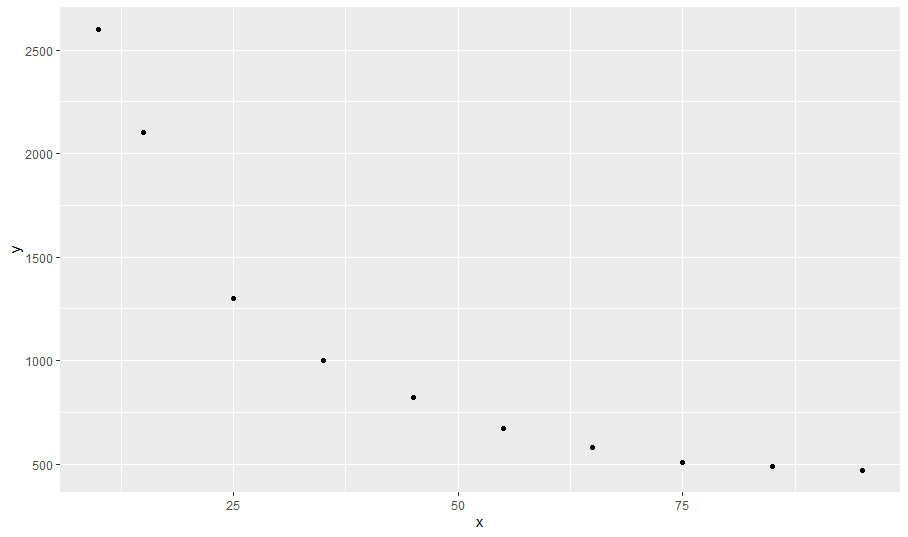
\includegraphics[width=\linewidth]{Plot.png}
  \caption{Точки на площині}
  \label{fig:image1}
\end{figure}

Помітимо, що це нагадує графік гіперболи, а тому зобразімо точки з координатами ($x$, $\frac{1}{y}$).

\begin{figure}[H]
  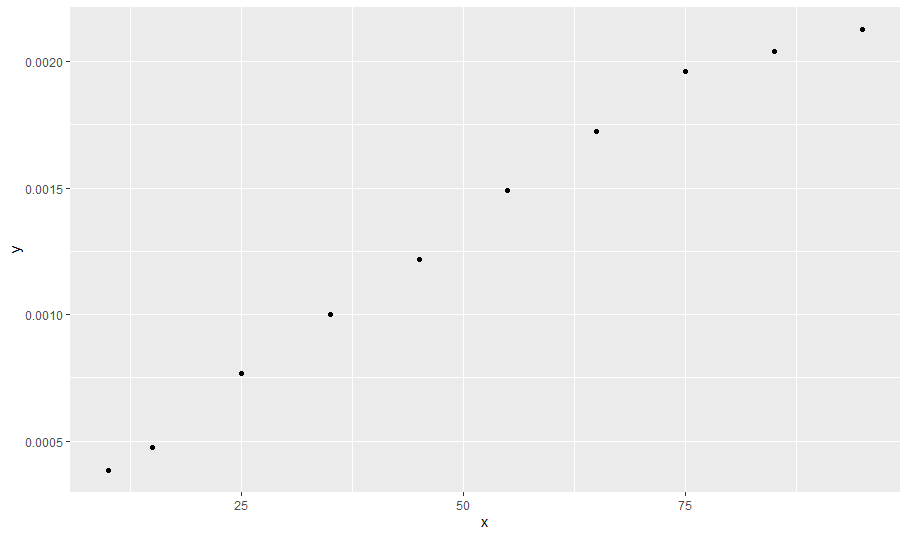
\includegraphics[width=\linewidth]{Inv_Plot.png}
  \caption{Точки на площині, де координати $y$ інверсовані}
  \label{fig:image2}
\end{figure}

Бачимо, що точки розташовані майже на прямій. Саме тому можна обрати вигляд функції, яку оцінює регресійна модель, як

\begin{align*}
  & f(x) = \frac{1}{\beta_{0} + \beta_{1} x}.
\end{align*}

Але цю модель можна спростити. Давайте будемо оцінювати функцію

\begin{align*}
  & g(x) = \frac{1}{f(x)}.
\end{align*}

Тоді

\begin{align*}
  & g(x) = \beta_{0} + \beta_{1} x.
\end{align*}

Одразу позначатимемо $\vec{\eta}^{(f)}$ - відклик або вихідна величина. Також введемо позначення $\eta_{i}^{(g)} = \frac{1}{\eta_{i}^{(f)}}$. Ці позначення дозволяють нам тимчасово забути про існування функції $f$. Тобто можно працювати з функцією $g$.

\subsection{Знаходження оцінок параметрів за методом найменших квадратів}

Метод найменших квадратів полягає у знаходженні таких значень параметрів $\beta_{0}$ та $\beta_{1}$, щоб мінімізувати значення

\begin{align*}
  & \sum_{i = 1}^{10} (\eta^{(g)}_{i} - g(x_{i}))^2.
\end{align*}

Відомо, що оцінкою методом найменших квадратів параметрів лінійної регресії є вектор

\begin{align*}
  & \vec{\beta}^{*} = (F^{T}F)^{-1}F^{T}\vec{\eta}^{(g)}, &\text{  де  } F \text{ - матриця плану.}
\end{align*}

В умовах нашої задачі

\begin{align*}
  & F = \begin{pmatrix}
    1 & 1 & 1 & 1 & 1 & 1 & 1 & 1 & 1 & 1 \\
    10 & 15 & 25 & 35 & 45 & 55 & 65 & 75 & 85 & 95  \\
  \end{pmatrix}^{T}
\end{align*}

і

\begin{align*}
  & \vec{\eta}^{(g)} =\begin{pmatrix}
    0.384 & 0.476 & 0.769 & 1 & 1.219 & 1.492 & 1.724 & 1.96 & 2.04 & 2.127 \\
  \end{pmatrix} \cdot 10^{-3}.
\end{align*}

Виконавши всі розрахунки, отримаємо, що

\begin{align*}
  & \vec{\beta}^{*}_ {val} = \begin{pmatrix}
    2.185826  \\
    0.2180424  \\
  \end{pmatrix} \cdot 10^{-4}.
\end{align*}

Отже, ми отримали оцінку параметрів регресійної моделі. Зобразімо на другому рисунку пряму, яку задають значення оцінок параметрів $\beta_{0}$ і $\beta_{1}$.

\begin{figure}[H]
  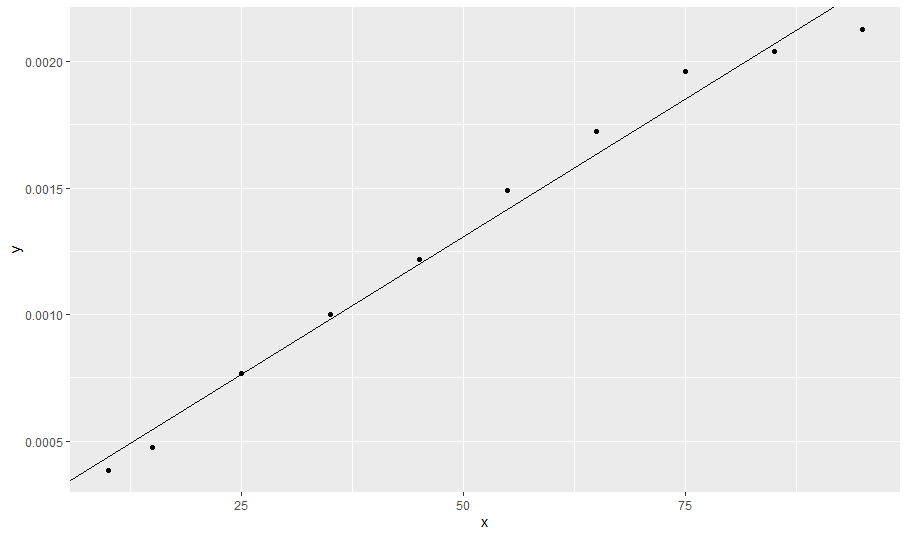
\includegraphics[width=\linewidth]{Plot_Line.png}
  \caption{Точки на площині та пряма}
  \label{fig:image3}
\end{figure}

\subsection{Перевірка адекватності побудованої моделі}

Висунемо нульову гіпотезу, що константа та побудована модель не відрізняються. Альтернативною оберемо гіпотезу, що побудована модель краща за константу.

Для перевірки адекватності побудованої моделі скористаємося $F$-критерієм - ми хочемо порівняти залишкову оцінку дисперсії з незміщеною оцінкою диспресії. Відомо, що статистика

\begin{align*}
  & \zeta = \frac{\frac{1}{n - 1} \sum_{i = 1}^{n} (\eta_{i}^{(g)} - \overline{\eta^{(g)}})^2}{\frac{1}{n - m} \sum_{i = 1}^{n} (\eta_{i}^{(g)} - g^{*}(x_{i}))^2} \sim F(n - 1, n - m),  & \text{  де  } m \text{ - кількість параметрів.}
\end{align*}

Вирахуємо значення, якими будемо користуватися згодом:

\begin{align*}
   & (\mathbb{D}^{**}\eta^{(g)})_{val} = \frac{1}{9} \sum_{i = 1}^{10} (y_{i}^{(g)} - \overline{y^{(g)}})^2 = 4.198214 \cdot 10^{-7}
\end{align*}

і

\begin{align*}
   & (\sigma_{(g)}^2)^{**}_{val} = \frac{1}{8} \sum_{i = 1}^{10} (y_{i}^{(g)} - g^{*}(x_{i}))^2 = 7.550273 \cdot 10^{-9}
\end{align*}

і

\begin{align*}
  & A^{-1} = F^{T}F = \begin{pmatrix}
    0.426 & -0.0064 \\
    -0.0064 & 0.00012  \\
  \end{pmatrix}.
\end{align*}

Надалі елементи матриці $A^{-1}$ позначатимемо маленькими літерами $a$ з індексами, якщо не вказано інше. Вирахуємо значення статистики.

\begin{align*}
  & \zeta_{val} = \frac{(\mathbb{D}^{**}\eta^{(g)})_{val}}{(\sigma_{(g)}^2)^{**}_{val}} = \frac{}{} = \frac{4.198214 \cdot 10^{-7}}{7.550273 \cdot 10^{-9}} = 55.603.
\end{align*}

На рівні значущості $\alpha = 0.05$ маємо $t_{cr} = 3.39$. Оскільки критична область правостороння і $\zeta_{val} > t_{cr}$, то нульову гіпотезу відхиляємо.

Отже, побудовану модель можна вважати адекватною.

\subsection{Перевірка гіпотези про значущість найменшого значення параметра побудованої моделі}

Оскільки ми з\textquotesingle ясували, що модель можна вважати адекватною, то перевіримо на значущість параметр $\beta_{0}$. Для цього висунемо нульову гіпотезу $H_{0}$ : $\beta_{0} = 0$. Альтернативна гіпотеза $H_{1}$ : $\beta_{0} > 0$.

Відомо, що статистика

\begin{align*}
  & \gamma^{(g)} = \frac{\beta_{0}^{*}}{\sqrt{(\sigma_{(g)}^2)^{**}\cdot a_{00}}} \sim St_{n - m}.
\end{align*}

Вирахуємо значення статистики.

\begin{align*}
  & \gamma^{(g)}_{val} = \frac{2.185826 \cdot 10^{-4}}{\sqrt{7.550273 \cdot 10^{-9} \cdot 0.426}} = 3.854.
\end{align*}

На рівні значущості $\alpha = 0.05$ маємо $t_{cr} = 1.86$. Оскільки критична область правостороння і $\zeta_{val} > t_{cr}$, то нульову гіпотезу відхиляємо.

Перевіримо на значущість і параметр $\beta_{1}$.

Для цього висунемо нульову гіпотезу $H_{0}$ : $\beta_{1} = 0$. Альтернативна гіпотеза $H_{1}$ : $\beta_{1} > 0$.

Відомо, що статистика

\begin{align*}
  & \gamma^{(g)} = \frac{\beta_{1}^{*}}{\sqrt{(\sigma_{(g)}^2)^{**}\cdot a_{11}}} \sim St_{n - m}.
\end{align*}

Вирахуємо значення статистики.

\begin{align*}
  & \gamma^{(g)}_{val} = \frac{0.2180424 \cdot 10^{-4}}{\sqrt{7.550273 \cdot 10^{-9} \cdot 0.0001}} = 25.09.
\end{align*}

На рівні значущості $\alpha = 0.05$ маємо $t_{cr} = 1.86$. Оскільки критична область правостороння і $\zeta_{val} > t_{cr}$, то нульову гіпотезу відхиляємо.

Отже, наша модель є адекватною і зменшити кількість параметрів не вдалося.

\begin{comment}
Нехай

\begin{align*}
  h(x) = \beta_{1} x.
\end{align*}

Перевіримо $h$ на адекватність. Для цього вирахуємо нові значення

\begin{align*}
   & (\mathbb{D}^{**}\eta^{(h)})_{val} = (\mathbb{D}^{**}\eta^{(g)})_{val} = 4.198214 \cdot 10^{-7}
\end{align*}

і

\begin{align*}
   & (\sigma_{(h)}^2)^{**}_{val} = \frac{1}{9} \sum_{i = 1}^{10} (y_{i}^{(h)} - h^{*}(\vec{x}^{(k)}))^2 = 5.97997 \cdot 10^{-8}.
\end{align*}

Вирахуємо значення аналогічної статистики $\zeta^{(h)}$.

\begin{align*}
  & \zeta^{(h)}_{val} = \frac{(\mathbb{D}^{**}\eta^{(h)})_{val}}{(\sigma_{(h)}^2)^{**}_{val}} = \frac{}{} = \frac{4.198214 \cdot 10^{-7}}{5.97997 \cdot 10^{-8}} = 7.02.
\end{align*}

На рівні значущості $\alpha = 0.05$ маємо $t_{cr} = 3.18$. Оскільки критична область правостороння і $\zeta^{(h)}_{val} > t_{cr}$, то нульову гіпотезу відхиляємо. Тобто модель $h$ можна вважати адекватною.

Перевіримо тепер параметр $\beta_{1}$ на значущість. Введемо аналогічну статистику, тільки тепер для функції $h$:

\begin{align*}
  & \gamma^{(h)} = \frac{\beta_{1}^{*}}{\sqrt{(\sigma_{(h)}^2)^{**}\cdot a_{11}}} \sim St_{n - m}.
\end{align*}

Вирахуємо значення статистики.

\begin{align*}
  & \gamma^{(h)}_{val} = \frac{2.185854 \cdot 10^{-4}}{\sqrt{5.97997 \cdot 10^{-8} \cdot 0.00012784}} = 79.05.
\end{align*}

На рівні значущості $\alpha = 0.05$ маємо $t_{cr} = 1.833$. Оскільки критична область правостороння і $\zeta_{val} > t_{cr}$, то нульову гіпотезу відхиляємо.

Отже, ми змогли спростити нашу модель до $h(x) = \beta_{1} x$.

\end{comment}

\subsection{Побудова прогнозованого довірчого інтервала для середнього значення відклику та самого значення відклику}

Повернімося до функції $f$.

\begin{align*}
  & f^{*}(x) = \frac{1}{g^{*}(x)} = \frac{1}{\beta^{*}_{0} +  \beta^{*}_{1} x}.
\end{align*}

Вирахуємо залишкову оцінку диспресії для $f$:

\begin{align*}
  & (\sigma_{(f)}^2)^{**}_{val} = \frac{1}{8} \sum_{i = 1}^{10} (y_{i}^{(f)} - f^{*}(x_{i}))^2 = 21512.43.
\end{align*}

Будемо будувати обидва довірчих інтервала для точки $\vec{x} = \begin{pmatrix}
  1 \\
  50\\
\end{pmatrix}$.

Знайдемо довірчий інтервал для середнього значення відклику. Відомо, що статистика

\begin{align*}
  \frac{f^{*}(x) - f(x)}{\vec{x}^\mathsf{T}A^{-1}\vec{x}} \sim St_{n - m}.
\end{align*}

Тоді довірчий інтервал для середнього значення відклику має вигляд

\begin{align*}
  & f(x) \in \left( f^{*}(x) - t \sqrt{(\sigma_{(f)}^2)^{**}_{val}  \vec{x}^\mathsf{T} A^{-1} \vec{x}}, f^{*}(x) + t \sqrt{(\sigma_{(f)}^2)^{**}_{val} \vec{x}^\mathsf{T} A^{-1} \vec{x}}  \right).
\end{align*}

Вирахуємо

\begin{align*}
  & \vec{x}^\mathsf{T}A^{-1}\vec{x} = 0.1, \\
  & \sqrt{(\sigma_{(f)}^2)^{**}_{val} \vec{x}^\mathsf{T} A^{-1} \vec{x}} = 46.38, \\
  & f^{*}(50) = \frac{1}{\beta^{*}_{0} +  \beta^{*}_{1} \cdot 50} = 764.1475.
\end{align*}

При рівні надійності $\gamma = 0.95$ маємо $t = t_{cr} = 2.306$. Підставлючи усі знайдені значення маємо, що

\begin{align*}
  & f(x) \in \left( 764.1475 - 2.306 \cdot 46.38, 764.1475 - 2.306 \cdot 46.38  \right) \Leftrightarrow f(x) \in \left( 657.19, 871.1  \right).
\end{align*}

Знайдемо довірчий інтервал для самого значення відклику. Відомо, що статистика

\begin{align*}
  & \frac{\eta - f^{*}(x)}{(\sigma_{(f)}^2)^{**} (1 + \vec{x}^\mathsf{T} A^{-1} \vec{x})} \sim St_{n - m}.
\end{align*}

Тому довірчий інтервал для середнього значення відклику має вигляд

\begin{align*}
  & \eta \in \left( f^{*}(x) - t\sqrt{(\sigma_{(f)}^2)^{**}_{val} (1 + \vec{x}^\mathsf{T} A^{-1} \vec{x}}), f^{*}(x) + t\sqrt{(\sigma_{(f)}^2)^{**}_{val} (1 + \vec{x}^\mathsf{T} A^{-1} \vec{x}})  \right).
\end{align*}

Акуратно підставивши значення отримаємо

\begin{align*}
  & \eta \in \left( 764.1475 - 2.306 \cdot 153.83, 764.1475 - 2.306 \cdot 153.83  \right) \Leftrightarrow \eta \in \left( 409.42, 1118.88  \right).
\end{align*}

\subsection{Висновок}

На момент аналізу даних у мене були думки щодо двух моделей. Після деяких спроб модифікації даних я отримав, що якщо значення $y$ замінити на обернені величини, то точки на графіку будут знаходитися майже на одній прямій. Таким чином можна було розглядати обернену функцію і будувати лінійну регресійну модель відштовхуючись від цього.

Після цих думок з\textquotesingle явилася думка, що можна задати вигляд функції $f$ як $f = \beta_{0} + \beta_{1} \cdot \frac{1}{x}$. Перевагою цією моделі від першої є те, що тут не потрібно переходити між функціями. Але я побудував графіки обох оцінок функцій - і мені здалося, що перша модель більш точно виражає поведінку даних. Саме тому модель виду $f(x) = \frac{1}{\beta_{0} + \beta_{1} x}$ була обрана для оцінки.

\newpage

\section{Задача 2}

\subsection{Постановка задачі}

\subsection{Пошук оцінок параметрів двофакторної регресійної моделі за методом найменших квадратів}

\subsection{Перевірка адекватності побудованої моделі}

\subsection{Перевірка гіпотези про значущість найменшого значення параметра побудованої моделі}

\subsection{Побудова прогнозованого довірчого інтервала для середнього значення відклику та самого значення відклику}

\subsection{Висновок}

\nocite{*}
\bibliography{ms2.bib}
%\cite{dirac}
\bibliographystyle{unsrt}

\end{document}
